\documentclass[conference]{IEEEtran}

% ---- Packages ----
\usepackage[utf8]{inputenc}
\usepackage[T1]{fontenc}
\usepackage{amsmath,amssymb,amsthm}
\usepackage{algorithmic}
\usepackage{algorithm}
\usepackage{booktabs}
\usepackage{multirow}
\usepackage{graphicx}
\usepackage{tikz}
\usetikzlibrary{matrix,positioning,fit,backgrounds,calc}
\usepackage{pgfplots}
\pgfplotsset{compat=1.18}
\usepackage{listings}
\usepackage{xcolor}
\usepackage{balance}
\usepackage{url}
\usepackage{cite}
\usepackage{hyperref}
\hypersetup{hidelinks}

% ---- Theorem environments ----
\newtheorem{theorem}{Theorem}
\newtheorem{property}{Property}
\newtheorem{definition}{Definition}

% ---- Listings style for SQL ----
\lstdefinestyle{sql}{
  language=SQL,
  basicstyle=\ttfamily\scriptsize,
  keywordstyle=\bfseries\color{blue!70!black},
  commentstyle=\itshape\color{green!50!black},
  stringstyle=\color{red!60!black},
  showstringspaces=false,
  breaklines=true,
  frame=single,
  framesep=2pt,
  xleftmargin=4pt,
  xrightmargin=4pt,
  aboveskip=6pt,
  belowskip=4pt,
  morekeywords={RETURNS,TABLE,RETURN,FUNCTION,NVARCHAR,DATETIME2,LTRIM,RTRIM,CREATE,WITH,UNION,ALL,SELECT,FROM,WHERE,INNER,JOIN,ON,AS,IN,TOP,AND,OR,IS,NULL,INT,MAX}
}

% ---- Pseudocode style ----
\lstdefinestyle{pseudo}{
  basicstyle=\ttfamily\scriptsize,
  keywordstyle=\bfseries,
  showstringspaces=false,
  breaklines=true,
  frame=single,
  framesep=2pt,
  xleftmargin=4pt,
  xrightmargin=4pt,
  aboveskip=6pt,
  belowskip=4pt,
  morekeywords={ALGORITHM,FOR,EACH,IN,IF,RETURN,WHERE,EXISTS}
}

% ---- C# style ----
\lstdefinestyle{csharp}{
  language=[Sharp]C,
  basicstyle=\ttfamily\scriptsize,
  keywordstyle=\bfseries\color{blue!70!black},
  commentstyle=\itshape\color{green!50!black},
  stringstyle=\color{red!60!black},
  showstringspaces=false,
  breaklines=true,
  frame=single,
  framesep=2pt,
  xleftmargin=4pt,
  xrightmargin=4pt,
  aboveskip=6pt,
  belowskip=4pt,
  morekeywords={var,async,await,string,IQueryable,Expression,Func,Task,bool,where},
  literate={=>}{{\textcolor{blue!70!black}{=>}}}{2}
}


\begin{document}

% ---- Title ----
\title{Database-Native Authorization for Human and Autonomous Principals: The SHRBAC Model}

\author{\IEEEauthorblockN{Ross Slaney}}

\maketitle

% ===========================================================================
% ABSTRACT
% ===========================================================================
\begin{abstract}
Enterprise applications must answer two authorization questions: ``can this principal act on this resource?'' (point check) and ``which resources can this principal access, filtered, sorted, and paginated?'' (list filtering). The latter is harder: it requires composing authorization with application-defined filtering, sorting, and pagination into a single efficient query. We present SHRBAC (Scoped Hierarchical Role-Based Access Control), an authorization model whose structural constraints---tree-structured resources, flat roles, non-recursive groups, and scoped temporal grants---make enforcement a composable database predicate with bounded cost, and whose polymorphic principals extend the same grant semantics to human users, service accounts, and autonomous agents. We formalize the model, prove soundness and completeness of an inline Table-Valued Function (TVF) enforcement, and show that under cursor pagination, bounded principal sets and grant multiplicity, and indexed nested-loop plans, per-page cost is $O(k \cdot D)$. Empirical evaluation on SQL Server 2022 at 1.2M resource nodes ($D{=}5$) and 1.5M ($D{=}10$) confirms $N$-independence across three orders of magnitude in dense-access workloads.
\end{abstract}

\begin{IEEEkeywords}
access control, RBAC, authorization, query composition, autonomous principals
\end{IEEEkeywords}

% ===========================================================================
% 1. INTRODUCTION
% ===========================================================================
\section{Introduction}

\subsection{The Problem}

Modern B2B SaaS applications require authorization systems that answer two fundamentally different questions:

\begin{enumerate}
\item \textbf{Point check}: ``Can principal $p$ perform action $a$ on resource $r$?''---a boolean decision.
\item \textbf{List filtering}: ``What resources of type $T$ can principal $p$ access, given search criteria $C$, sorted by $S$, paginated to page $k$?''---a set-returning query integrated with application data.
\end{enumerate}

The first is well-understood: Google's Zanzibar~\cite{zanzibar} and its descendants handle millions of point checks per second through graph traversal and caching. The second---the \textbf{list filtering problem}---is trivial for flat access models (\texttt{WHERE tenant\_id = @currentTenant} composes directly) but becomes substantially harder when access derives from grants at varying hierarchy levels, resolved through group memberships, under temporal constraints.

Increasingly, principals are not only human users but \textbf{autonomous AI agents} that enumerate and filter large resource sets in loops. SHRBAC introduces no agent-specific policy semantics; it treats agents as first-class principals, so the same scoped, temporal grant model applies to human and autonomous callers, and the \textbf{principle of least privilege}~\cite{saltzer} is enforced structurally: narrow grants (specific subtree, limited role, bounded duration) guard against broad, long-lived authority.

When authorization logic resides outside the database, an impedance mismatch arises. Industry bridges this gap through ID lookups, batch post-filtering, partial policy evaluation, or materialized permission views---each trading scalability, consistency, or complexity. SHRBAC instead chooses structural constraints so that per-page enforcement cost is $O(k \cdot D)$ under bounded local parameters---linear in page size and tree depth, independent of total resource count $N$ and policy set size.

\textbf{Notation.} Throughout the paper, $N$ denotes total entities or resource nodes under evaluation, $k$ the requested page size, $D$ the maximum resource-tree depth, $M=|\mathit{resolve}(p)|$ the number of effective principals for caller $p$, $G_{\max}$ the maximum active grant multiplicity for the same principal-resource pair, and $\sigma$ the selectivity of authorized rows.

\subsection{Contributions}

\begin{enumerate}
\item \textbf{Constraint-driven model.} We introduce SHRBAC, whose four structural constraints---tree-structured resources, non-recursive principal groups, flat roles, and scoped temporal grants (principal $\times$ role $\times$ resource $\times$ time)---are deliberately chosen so that enforcement admits a fixed, schema-level relational artifact with bounded cost independent of policy set size. Polymorphic principals make users, groups, service accounts, and autonomous agents first-class grant recipients with least-privilege, time-bounded authority.

\item \textbf{Formalization with proved enforcement.} Access evaluation is two-dimensional---upward over a bounded-depth resource tree, outward over effective principals. We realize enforcement as a single inline Table-Valued Function \texttt{EXISTS} predicate defined at schema time and prove it sound and complete; grants are data rows, not predicate terms, requiring no runtime compilation, post-filtering, or external graph traversal.

\item \textbf{Complexity theorem for list filtering.} Per-row cost is bounded at $O(D \cdot M \cdot G_{\max})$; under cursor pagination, per-page cost is $O(k \cdot D)$ when $M$ and $G_{\max}$ are bounded---independent of resource count $N$, policy set size, and page depth. This formal bound for the list-filtering problem is absent in prior RBAC, ABAC, and ReBAC models.

\item \textbf{Production-scale empirical validation.} At 1.2M resources ($D{=}5$) and 1.5M resources ($D{=}10$), we confirm $N$-independence across three orders of magnitude, linear scaling in $k$ and $D$, constant per-CTE-hop cost, cursor-depth independence, and grant-breadth independence in tested dense-access workloads.
\end{enumerate}

% ===========================================================================
% 2. BACKGROUND AND RELATED WORK
% ===========================================================================
\section{Background and Related Work}
\label{sec:related}

\subsection{RBAC Foundations}

Sandhu et al.~\cite{rbac96} defined the RBAC96 family: RBAC0 (core), RBAC1 (hierarchical roles), RBAC2 (constraints), and RBAC3 (combined). The NIST standard~\cite{nist-rbac} formalized Core and Hierarchical RBAC. \textbf{Critical gap:} RBAC96 defines only a role hierarchy; the resource space is flat with no concept of resource hierarchy or scope.

\subsection{Hierarchical Models}

\textbf{ROBAC} (Zhang et al.~\cite{robac}) introduced the (user, role, organization) triple with grants cascading down an organization hierarchy. SHRBAC's (principal, role, resource) grant is structurally identical, but ROBAC defines a policy semantics without constraining the model to admit a fixed enforcement artifact with bounded evaluation cost. SHRBAC's novelty is the alignment of model constraints with relational query-planning guarantees, extended to polymorphic principals. \textbf{RRBAC} (Solanki et al.~\cite{rrbac}) formalized resource hierarchies with grant cascade but did not address polymorphic principals, query composition, or enforcement mechanisms. \textbf{OrBAC} (Kalam et al.~\cite{orbac}) generalized RBAC with five hierarchies; its expressiveness exceeds what TVF-based enforcement requires---SHRBAC is a practical engineering subset.

\subsection{Query Modification and Enforcement}

Stonebraker and Wong~\cite{stonebraker} introduced query modification for INGRES---the ancestor of Oracle VPD and SQL Server/PostgreSQL row-level security. Rizvi et al.~\cite{rizvi} distinguished the \emph{Truman model} (silent filtering, which SHRBAC implements) from the \emph{Non-Truman model} (query rejection). Pappachan et al.~\cite{sieve} showed that naive predicate injection does not scale with thousands of policies; SHRBAC's predicate is a single TVF invocation regardless of policy count.

\subsection{Zanzibar, ReBAC, and List Filtering}

Google's Zanzibar~\cite{zanzibar} uses relationship tuples with a userset rewrite system; Fong~\cite{fong} formalized ReBAC using modal logic. Zanzibar's \texttt{tuple\_to\_userset} handles resource hierarchies through general graph traversal. SHRBAC constrains resources to a tree and uses typed roles rather than arbitrary relation composition---tree traversal has bounded depth, which is what makes TVF enforcement tractable. Composing authorization into list queries has no canonical academic name: vendors call it ``ACL-aware filtering,'' ``list filtering,'' or a ``query plan'' problem~\cite{vendor-docs}. At scale, SpiceDB recommends progressively more complex strategies (LookupResources $\to$ CheckBulkPermissions $\to$ Materialize). SHRBAC is designed so that the integration surface is a relational predicate---composable by construction.

\subsection{Summary of Gaps}

Table~\ref{tab:gaps} summarizes the capability comparison. To our knowledge, no prior model jointly formalizes resource hierarchy with grant cascade, polymorphic principals (humans, groups, and agents as first-class grant recipients), and a concrete query-composable enforcement mechanism with a complexity bound.

\begin{table*}[t]
\centering
\caption{Capability comparison across authorization models. ``\checkmark'' indicates native support.}
\label{tab:gaps}
\scriptsize
\begin{tabular}{@{}lcccccc@{}}
\toprule
\textbf{Capability} & \textbf{RBAC96} & \textbf{ROBAC} & \textbf{RRBAC} & \textbf{OrBAC} & \textbf{ReBAC} & \textbf{SHRBAC} \\
\midrule
Role hierarchy         & RBAC1+ & \checkmark & \checkmark & \checkmark & N/A & No (flat) \\
Resource hierarchy     & No & Org hier. & \checkmark & Org hier. & Graph & \checkmark{} (tree) \\
Grant cascade          & No & \checkmark & \checkmark & \checkmark & \texttt{tuple\_to\_userset} & \checkmark \\
Polymorphic principals & No & No & No & Partial & Usersets & \checkmark \\
Group-as-principal     & No & No & No & No & Via tuples & \checkmark \\
Agent-as-principal     & No & No & No & No & No & \checkmark \\
Temporal grants        & No & No & No & Contexts & No & \checkmark \\
Query composition      & No & No & No & No & No & \checkmark \\
Formal enforcement     & No & No & No & No & Graph trav. & Query mod. \\
\bottomrule
\end{tabular}
\end{table*}

% ===========================================================================
% 3. THE SHRBAC MODEL
% ===========================================================================
\section{The SHRBAC Model}
\label{sec:model}

\subsection{Basic Sets}

The model comprises: a finite set $\mathcal{P}$ of \emph{principals}, each typed $\tau(p) \in \{\text{user}, \text{group}, \text{service\_account}, \text{agent}\}$, where an agent is an autonomous process (AI agent, orchestration pipeline, or background service) participating in the same grant relation as human users under the same scoping and temporal constraints; a finite set $\mathcal{R}$ of \emph{roles}; a finite set $\mathit{PERM}$ of atomic \emph{permissions} (e.g., \textsc{project\_view}); a finite set $\mathit{RES}$ of \emph{resources} forming nodes in a rooted tree, each carrying a type from $\mathit{RT}$ (e.g., \texttt{portal\_root}, \texttt{agency}, \texttt{project}); and the time domain $\mathcal{T}$ (UTC timestamps).

\subsection{Resource Hierarchy}

The resource hierarchy is a rooted tree $(\mathit{RES}, \mathit{parent})$ with $\mathit{parent}: \mathit{RES} \to \mathit{RES} \cup \{\bot\}$ and $\mathit{parent}(r_0) = \bot$ for the root $r_0$. Define $\mathit{ancestors}(r) = \{\mathit{parent}^i(r) \mid i \geq 0 \wedge \mathit{parent}^i(r) \neq \bot\}$ (note $r \in \mathit{ancestors}(r)$), $\mathit{descendants}(r) = \{r' \in \mathit{RES} \mid r \in \mathit{ancestors}(r')\}$, and $\mathit{depth}(r) = |\mathit{ancestors}(r)| - 1$. The tree is bounded: $\mathit{depth}(r) \leq D$ for all $r$; in practice $D = 3$--$5$ for typical SaaS and up to $10$--$15$ for deep enterprise hierarchies. An \textbf{authorized entity} is a row in an application table carrying a \texttt{ResourceId} referencing a node in the resource tree.

\subsection{Role-Permission Assignment}

$PA \subseteq \mathcal{R} \times \mathit{PERM}$ is the role-permission assignment. Each permission has an associated resource type: $\mathit{applicable}: \mathit{PERM} \to \mathit{RT}$. Roles are \textbf{flat}---no role hierarchy. The resource hierarchy provides the inheritance dimension, avoiding the combinatorial complexity of dual hierarchies.

\subsection{Principal Resolution}

Groups are themselves principals. $\mathit{members}(g) = \{u \in \mathcal{P} \mid \tau(u) = \text{user} \wedge u \text{ is a member of } g\}$. Membership is not recursive---groups cannot contain other groups.

\textbf{Principal resolution} expands a user to their effective principal identities:
\[
\mathit{resolve}(p) = \{p\} \cup \{g \in \mathcal{P} \mid \tau(g) = \text{group} \wedge p \in \mathit{members}(g)\}
\]

For non-user principals (groups, service accounts, agents), $\mathit{resolve}(p) = \{p\}$.

\subsection{Grants}

$G \subseteq \mathcal{P} \times \mathcal{R} \times \mathit{RES} \times (\mathcal{T} \cup \{\bot\}) \times (\mathcal{T} \cup \{\bot\})$

A grant $g = (p, \mathit{role}, \mathit{res}, t_{\mathit{from}}, t_{\mathit{to}})$ assigns role $\mathit{role}$ to principal $p$ at resource $\mathit{res}$, effective during the closed (inclusive) interval $[t_{\mathit{from}}, t_{\mathit{to}}]$; a $\bot$ bound means unbounded.

\textbf{Active grants} at time $t$:
\begin{multline*}
\mathit{active}(t) = \{(p, \mathit{role}, \mathit{res}) \mid (p, \mathit{role}, \mathit{res}, t_f, t_t) \in G \\
\wedge\; (t_f = \bot \vee t_f \leq t) \wedge (t_t = \bot \vee t_t \geq t)\}
\end{multline*}

The grant triple (principal, role, resource) enforces least privilege: authority is scoped to a specific subtree (not global), a specific role (not all permissions), and optionally a specific time window (not permanent).

\subsection{Access Evaluation Function}

\begin{definition}[Access Decision]
Given principal $p$, permission $\mathit{perm}$, resource $r$, and time $t$:
\begin{multline*}
\mathit{allowed}(p, \mathit{perm}, r, t) = \exists\, p' \in \mathit{resolve}(p),\\
\exists\, r' \in \mathit{ancestors}(r),\; \exists\, \mathit{role} \in \mathcal{R}: \\
(p', \mathit{role}, r') \in \mathit{active}(t) \wedge \mathit{perm} \in \mathit{perms}(\mathit{role})
\end{multline*}
\end{definition}

Access is granted if \emph{any} effective identity has \emph{any} active grant at \emph{any} ancestor of the target resource with a role including the requested permission. This is \textbf{two-dimensional resolution}: simultaneously walking UP the resource tree and expanding OUT the principal set.

\textbf{Running example.} Let \texttt{portal\_root} $\to$ \texttt{agency\_7} $\to$ \texttt{project\_42}, with Alice in group \texttt{engineering} and a single grant (\texttt{engineering}, \textsc{Viewer}, \texttt{agency\_7}). Evaluating $\mathit{allowed}(\text{alice}, \textsc{project\_view}, \texttt{project\_42}, \mathit{now})$ searches the $2 \times 3$ grid $\mathit{resolve}(\text{alice}) \times \mathit{ancestors}(\texttt{project\_42})$ and finds the \textsc{Viewer} grant at (\texttt{engineering}, \texttt{agency\_7}): access is granted---the grant cascades to the descendant \texttt{project\_42} (Fig.~\ref{fig:resolution}).

% ---- FIGURE: Two-dimensional resolution grid ----
\begin{figure}[t]
\centering
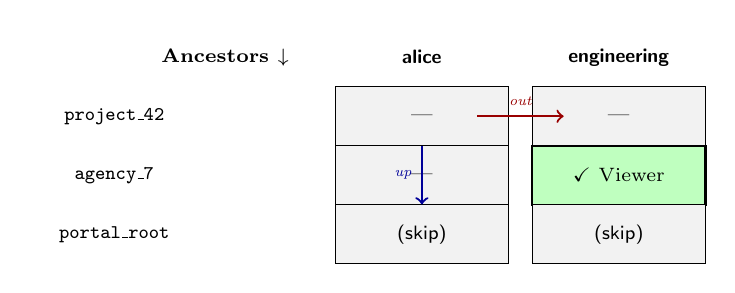
\begin{tikzpicture}[
  cell/.style={minimum width=2.2cm, minimum height=0.75cm, draw, font=\scriptsize, anchor=center},
  header/.style={minimum width=2.2cm, minimum height=0.75cm, font=\scriptsize\bfseries, anchor=center},
  match/.style={cell, fill=green!25, thick},
  miss/.style={cell, fill=gray!10},
]

% Column headers
\node[header] at (0, 3.0) {Ancestors $\downarrow$};
\node[header] at (2.5, 3.0) {\textsf{alice}};
\node[header] at (5.0, 3.0) {\textsf{engineering}};

% Row 1: project_42
\node[header, anchor=east] at (-0.3, 2.25) {\texttt{project\_42}};
\node[miss] at (2.5, 2.25) {---};
\node[miss] at (5.0, 2.25) {---};

% Row 2: agency_7
\node[header, anchor=east] at (-0.3, 1.5) {\texttt{agency\_7}};
\node[miss] at (2.5, 1.5) {---};
\node[match] at (5.0, 1.5) {\checkmark{} Viewer};

% Row 3: portal_root
\node[header, anchor=east] at (-0.3, 0.75) {\texttt{portal\_root}};
\node[miss] at (2.5, 0.75) {\textsf{(skip)}};
\node[miss] at (5.0, 0.75) {\textsf{(skip)}};

% Arrows
\draw[->, thick, blue!60!black] (2.5, 1.87) -- (2.5, 1.13) node[midway, left, font=\tiny\itshape] {up};
\draw[->, thick, red!60!black] (3.2, 2.25) -- (4.3, 2.25) node[midway, above, font=\tiny\itshape] {out};

\end{tikzpicture}
\caption{Two-dimensional resolution for the running example: principals expand outward (columns), ancestors are walked upward (rows), and the first match short-circuits.}
\label{fig:resolution}
\end{figure}

\subsection{Properties}

\begin{property}[Monotonicity of Hierarchy]
If $\mathit{allowed}(p, \mathit{perm}, r, t)$ and $r' \in \mathit{descendants}(r)$, then the same grant provides access at $r'$ (immediate from transitivity of the ancestor relation).
\end{property}

\begin{property}[Monotonicity of Groups]
Adding $p$ to group $g$ preserves existing access and may grant additional access (existential quantification over an expanded $\mathit{resolve}(p)$).
\end{property}

\begin{property}[Bounded Evaluation]
For any access decision, evaluation examines at most $|\mathit{resolve}(p)| \times |\mathit{ancestors}(r)| \times G_{\max}$ grant entries, giving $O(M \cdot D \cdot G_{\max})$.
\end{property}

% ===========================================================================
% 4. QUERY-COMPOSABLE ENFORCEMENT VIA TVF
% ===========================================================================
\section{Query-Composable Enforcement via TVF}
\label{sec:tvf}

\subsection{The Table-Valued Function}

The enforcement mechanism realizes Definition~1 directly as an inline Table-Valued Function (iTVF), evaluated per row as an \texttt{EXISTS} predicate:

\begin{lstlisting}[style=sql]
CREATE FUNCTION dbo.fn_IsResourceAccessible(
  @ResourceId NVARCHAR(128), @PrincipalIds NVARCHAR(MAX),
  @PermissionId NVARCHAR(128), @Now DATETIME2)
RETURNS TABLE AS RETURN (
  WITH ancestors AS (
    SELECT Id, ParentId, 0 AS Depth
      FROM Resources WHERE Id = @ResourceId
    UNION ALL
    SELECT r.Id, r.ParentId, a.Depth + 1
      FROM Resources r
      INNER JOIN ancestors a ON r.Id = a.ParentId
      WHERE a.Depth < 10)
  SELECT TOP 1 a.Id FROM ancestors a
    INNER JOIN Grants g ON a.Id = g.ResourceId
    INNER JOIN RolePermissions rp ON g.RoleId = rp.RoleId
  WHERE g.PrincipalId IN (SELECT LTRIM(RTRIM(value))
          FROM STRING_SPLIT(@PrincipalIds, ','))
    AND rp.PermissionId = @PermissionId
    AND (g.EffectiveFrom IS NULL OR g.EffectiveFrom <= @Now)
    AND (g.EffectiveTo IS NULL OR g.EffectiveTo >= @Now))
\end{lstlisting}

The recursive CTE walks UP from the target resource to the root (at most $D$ levels), joining against active grants at each ancestor. \texttt{TOP 1} provides existential semantics---one matching grant suffices. The caller-controlled \texttt{@Now} parameter ensures deterministic evaluation across all rows in a query. As an inline TVF, the optimizer composes its body into the calling query's execution plan: the application layer resolves group memberships once per request, then appends the TVF as an \texttt{EXISTS} predicate alongside application-defined filters, cursor pagination, and sorting---authorization and application logic execute as a single database operation, one round-trip, zero external calls. We use SQL Server as an exemplar because its optimizer aggressively inlines iTVFs; the enforcement requires only recursive CTEs and predicate inlining, both supported by PostgreSQL and other modern engines.

\subsection{Correctness}

\begin{theorem}[Soundness and Completeness]
For entities with $\mathit{depth} \leq 10$, the TVF returns a non-empty result for entity $e$ iff $\mathit{allowed}(p, \mathit{perm}, e.\mathit{ResourceId}, \mathit{now}) = \text{true}$.
\end{theorem}
\begin{proof}
The recursive CTE (guard \texttt{Depth~$<$~10}) produces exactly $\mathit{ancestors}(e.\mathit{ResourceId})$; the joins against \texttt{Grants} and \texttt{RolePermissions} with the temporal predicates implement the existential quantification of Definition~1 over $\mathit{active}(t)$. A non-empty result therefore witnesses a satisfying $(p', \mathit{role}, r')$ triple, and conversely any satisfying witness matches the corresponding CTE row, principal filter, and temporal and role-permission predicates by construction.
\end{proof}

% ===========================================================================
% 5. COMPLEXITY ANALYSIS
% ===========================================================================
\section{Complexity Analysis}
\label{sec:complexity}

\subsection{Per-Row TVF Cost}

For a single entity with resource at depth $d \leq D$, the CTE performs $O(D)$ index seeks on \texttt{Resources(Id)}; joining the $D$ ancestors against \texttt{Grants} and \texttt{RolePermissions} examines at most $D \cdot M \cdot G_{\max}$ candidates; and \texttt{TOP 1} short-circuits on the first match. \textbf{Per-row cost:} $O(D \cdot M \cdot G_{\max})$---with $D = 5$, $M = 10$, $G_{\max} = 3$, ${\sim}150$ index lookups.

\subsection{Per-Page Cost Under Pagination}

\begin{theorem}[Per-Page Complexity]
\label{thm:perpage}
Assume (1) index coverage on Resources, Grants, RolePermissions, and entity ResourceId; (2) cursor pagination on an indexed ordering key; (3) nested-loops plans with index seeks. Then dense access ($\sigma \approx 1$) costs $O(k \cdot D \cdot M \cdot G_{\max})$ per page---$O(k \cdot D)$ when $M$ and $G_{\max}$ are bounded constants---and sparse access costs $O(k/\sigma \cdot D \cdot M \cdot G_{\max})$, degenerating to $O(N \cdot D \cdot M \cdot G_{\max})$ when no rows are authorized.
\end{theorem}
\begin{proof}
With cursor pagination the engine seeks to the cursor in $O(\log N)$ and evaluates candidates sequentially, each costing $O(D \cdot M \cdot G_{\max})$ by the per-row bound above; collecting $k$ authorized rows at selectivity $\sigma$ examines ${\sim}k/\sigma$ candidates, giving $O(k/\sigma \cdot D \cdot M \cdot G_{\max})$. The cursor start is resolved by index seek, not by scanning prior pages, so cost is independent of page depth and $N$.
\end{proof}

The per-page cost is \emph{parameterized and predictable}---independent of $N$, linear in $D$. Alternatives instead pay an external-service round trip per page (LookupResources, batch post-filtering), a policy-compilation step (partial evaluation), or eventual-consistency denormalization infrastructure (materialized views); SHRBAC's cost is database-local with strong consistency.

% ===========================================================================
% 7. EMPIRICAL EVALUATION
% ===========================================================================
\section{Empirical Evaluation}
\label{sec:empirical}

We evaluate SHRBAC on SQL Server 2022 (Docker, 4 vCPU, 8~GB RAM) across three tiers: (1)~small-scale isolation tests (1K--100K entities) that individually vary each factor, (2)~a production-scale workload at $D{=}5$ with 1.2M resource nodes, and (3)~a deep-hierarchy workload at $D{=}10$ with 1.5M resource nodes. The environment is a controlled validation setup, not a production latency claim; Section~\ref{sec:discussion} discusses generalizability.

\subsection{Benchmark Methodology}

\textbf{Measurement protocol.} Each query: 3 warmup runs (discarded), 20 measured runs, each on a fresh connection, recording wall-clock elapsed time. We report median and P95. Page size $k = 20$ unless stated otherwise.

\textbf{Query pattern.} All list-filtering benchmarks execute the canonical authorized-list query: select the top $k$ \texttt{Products} rows satisfying \texttt{EXISTS(fn\_IsResourceAccessible(\ldots))} with a cursor predicate (\texttt{Id > @cursor}) and \texttt{ORDER BY Id}. Point checks use the same TVF against a single ResourceId. Query plans were verified to use nested loops with index seeks.

\textbf{Principal parameter passing.} All reported benchmarks, including the $M{=}11$ and $M{=}21$ experiments, use the \texttt{STRING\_SPLIT} TVF of Section~\ref{sec:tvf} (no table-valued parameters), so $M$-scaling conclusions are limited to the tested range. \texttt{STRING\_SPLIT} can produce poor cardinality estimates; table-valued parameters are recommended for larger principal sets.

\textbf{Hierarchies.} $D{=}5$: root $\to$ 15 chains $\to$ 150 regions $\to$ 15K stores $\to$ 1.2M products = \textbf{1,215,166 resources}. $D{=}10$: root $\to$ 5 divisions $\to$ 25 regions $\to$ 125 districts $\to$ 500 areas $\to$ 2K zones $\to$ 12K stores $\to$ 60K departments $\to$ 240K sections $\to$ 1.2M products = \textbf{1,514,656 resources}. Resources and domain rows are bulk-inserted; \texttt{UPDATE STATISTICS} is run before benchmarks.

\textbf{Isolation tests} (Benchmarks 1--7) use the same retail domain model scaled to the target depth (e.g., $D{=}3$: root $\to$ Regions $\to$ Stores $\to$ Products($N$)). Each level is a real domain table whose rows map to unique resources, and the benchmark query always targets Products, so small-scale tests exercise the same schema and query patterns as the production-scale ones.

\subsection{Isolation Tests (1K--100K)}

Controlled single-factor experiments, re-seeded per configuration, confirm the core predictions: $N$-independence across 1K--100K (3.32--3.57ms median at $D{=}3$; Fig.~\ref{fig:scaling}), monotonic depth scaling from 2.45ms ($D{=}1$) through 3.17ms ($D{=}3$) to 4.21ms ($D{=}5$) consistent with $O(k \cdot D)$, and a negligible principal-set effect (3.32--3.47ms across $M{=}1$--$21$). P95 stayed below 6.2ms in every configuration.

% ---- FIGURE: N-independence across three orders of magnitude ----
\begin{figure}[t]
\centering
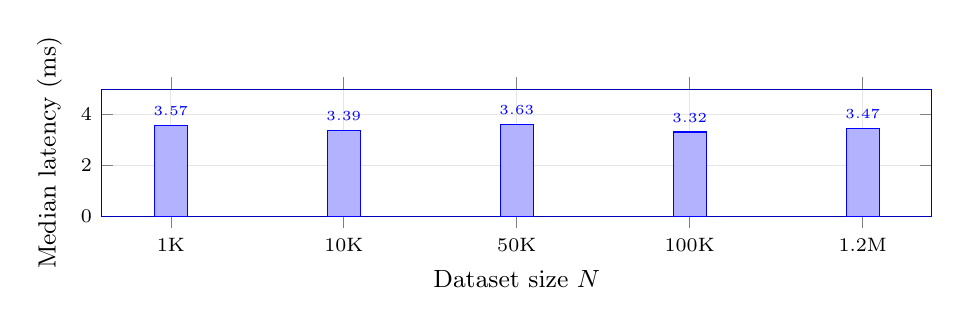
\begin{tikzpicture}
\begin{axis}[
    width=\columnwidth,
    height=3.2cm,
    xlabel={Dataset size $N$},
    ylabel={Median latency (ms)},
    symbolic x coords={1K,10K,50K,100K,1.2M},
    xtick=data,
    ymin=0, ymax=5,
    ybar,
    bar width=12pt,
    nodes near coords,
    nodes near coords style={font=\tiny},
    every node near coord/.append style={above},
    grid=major,
    grid style={gray!20},
    every axis label/.style={font=\small},
    every tick label/.style={font=\scriptsize},
    fill=blue!50,
    draw=blue!70!black,
]
\addplot coordinates {(1K, 3.57) (10K, 3.39) (50K, 3.63) (100K, 3.32) (1.2M, 3.47)};
\end{axis}
\end{tikzpicture}
\caption{Per-page median latency ($k{=}20$, cursor) is flat at ${\sim}$3.3--3.6ms across three orders of magnitude; the small increase at 1.2M is a depth effect ($D{=}5$ vs $D{=}3$), not resource count.}
\label{fig:scaling}
\end{figure}

\subsection[Production-Scale at D=5 (1.2M Resources)]{Production-Scale at $D{=}5$ (1.2M Resources)}

Principals range from company administrators (all 1.2M products accessible) to store managers (${\sim}$80 products); page-size results appear in Table~\ref{tab:d10}. \textbf{Scope level}: despite a $15{,}000\times$ difference in accessible product count, latency varies minimally---company admin 3.47ms, chain manager 3.20ms, region manager 3.11ms, store manager 2.02ms median (P95 $\leq$ 6.34ms)---store-level grants fastest because the CTE short-circuits. \textbf{Cursor depth} is flat: 3.08ms at page~1, 3.25ms at page~50, 3.48ms at page~500.

\subsection[Deep Hierarchy at D=10 (1.5M Resources)]{Deep Hierarchy at $D{=}10$ (1.5M Resources)}

Table~\ref{tab:d10} compares identical queries across both tree depths.

\begin{table}[t]
\centering
\caption{Page size comparison: $D{=}5$ vs.\ $D{=}10$.}
\label{tab:d10}
\scriptsize
\begin{tabular}{@{}lrrr@{}}
\toprule
$k$ & \textbf{$D{=}5$ (ms)} & \textbf{$D{=}10$ (ms)} & \textbf{Ratio} \\
\midrule
10 & 2.28 & 3.44 & 1.51$\times$ \\
20 & 3.47 & 5.69 & 1.64$\times$ \\
50 & 6.89 & 11.80 & 1.71$\times$ \\
100 & 13.71 & 22.01 & 1.61$\times$ \\
\bottomrule
\end{tabular}
\end{table}

Page size scales linearly at both depths: $k{=}10 \to 100$ yields $6.01\times$ at $D{=}5$ and $6.40\times$ at $D{=}10$, closely tracking $O(k)$. The $D{=}10$/$D{=}5$ ratio (1.51--1.71$\times$) is below the theoretical $9/4 = 2.25\times$ because fixed per-page overhead is proportionally larger at $D{=}5$; the gap narrows at larger $k$. Per-row cost is ${\sim}$0.14ms at $D{=}5$ (${\sim}$0.034ms per CTE hop) and ${\sim}$0.22ms at $D{=}10$ (${\sim}$0.024ms per hop), giving $O(k \cdot D)$ a concrete, measurable constant. Scope-level and cursor-depth results at $D{=}10$ mirror $D{=}5$: scope varies minimally (3.06--5.54ms), and cursor depth is flat (5.11--5.38ms across pages 1--500).

\subsection{Point Access Checks}

The TVF also serves as a point check. Across target depths 0--4 at $D{=}5$ (1.2M resources), point checks complete in 0.86--1.31ms median; across depths 0--9 at $D{=}10$ (1.5M resources), in 0.89--1.46ms---all \textbf{under 1.5ms median} even at depth~9. Grant set size (1--20 active grants; 1.19--1.38ms) and principal set size ($M{=}1$--$21$; 0.98--1.28ms) are flat in the tested \texttt{STRING\_SPLIT} range. The CTE examines only the target resource's ancestor chain (${\leq}D$ nodes), not the grant table at large.

\subsection{Analysis}

\textbf{$N$-independence extends to 1.5M resources (Fig.~\ref{fig:scaling}).} With 1,215,166 unique resource nodes at $D{=}5$, list filtering median is 3.47ms ($k{=}20$)---compared to 3.39ms at $N{=}$10K with $D{=}3$ in isolation tests. The small increase is attributable to depth, not resource count. At $D{=}10$ with 1,514,656 resources, per-page cost is 5.69ms---again a depth effect.

\textbf{Grant breadth is not local grant multiplicity.} The breadth experiments vary the number of distinct resource scopes granted to a principal: at $D{=}5$, 1 vs.\ 10 chain scopes changes median latency by 0.09ms (3.31 vs.\ 3.40ms); at $D{=}10$, 1 vs.\ 5 division scopes changes it from 5.00ms to 5.76ms. Unrelated grant rows at other scopes are not scanned when evaluating a candidate resource. $G_{\max}$---multiple active grants for the same principal-resource pair---is a different factor: point checks showed no sensitivity for 1--20 active grants, though the evaluation does not refute the formal $O(G_{\max})$ factor.

\textbf{Narrow grants can improve constants.} A chain-level grant (3.12ms) is 37\% slower than a single store grant (2.28ms): the CTE walks UP from the product, so a store-level grant matches at the first ancestor hop while a chain-level grant requires 3--4 hops. The 100-store case (4.27ms vs.\ 2.50ms for 10 stores) shows many disjoint narrow grants are not monotonically faster; selectivity and plan estimates affect constants without violating the per-row bound.

\textbf{Principal set size is negligible in the tested range.} $M{=}1$ vs $M{=}11$ produces 3.36 vs.\ 3.44ms ($D{=}5$) and 5.63 vs.\ 5.85ms ($D{=}10$). Because these experiments used \texttt{STRING\_SPLIT}, this is an empirical observation for small effective-principal sets ($M \leq 21$), not a claim that parameter passing is irrelevant for large $M$.

\textbf{Cursor vs.\ offset pagination (Fig.~\ref{fig:pagination}).} Offset COUNT costs grow linearly with $N$ while cursor pagination remains at ${\sim}$3.3ms: $700\times$ faster at $N{=}$100K.

% ---- FIGURE: Cursor vs Offset pagination ----
\begin{figure}[t]
\centering
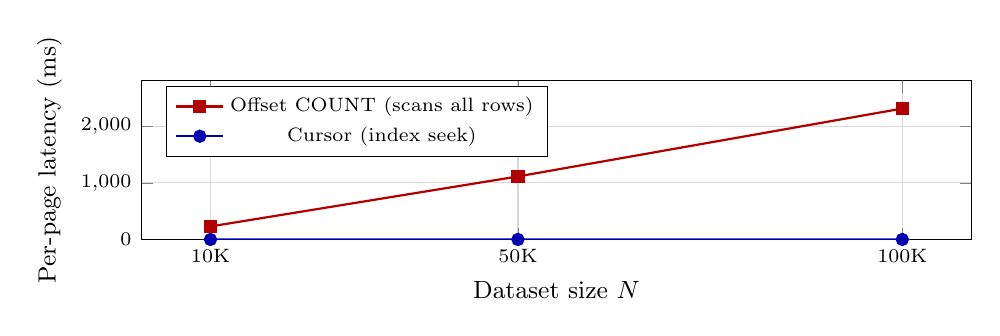
\begin{tikzpicture}
\begin{axis}[
    width=\columnwidth,
    height=3.6cm,
    xlabel={Dataset size $N$},
    ylabel={Per-page latency (ms)},
    xtick={10000,50000,100000},
    xticklabels={10K,50K,100K},
    scaled x ticks=false,
    ymin=0, ymax=2800,
    legend style={at={(0.03,0.97)}, anchor=north west, font=\scriptsize},
    grid=major,
    grid style={gray!30},
    every axis label/.style={font=\small},
    every tick label/.style={font=\scriptsize},
]

% Offset line
\addplot[
    color=red!70!black,
    mark=square*,
    thick,
    mark size=2pt,
] coordinates {
    (10000, 233)
    (50000, 1114)
    (100000, 2310)
};
\addlegendentry{Offset COUNT (scans all rows)}

% Cursor line
\addplot[
    color=blue!70!black,
    mark=*,
    thick,
    mark size=2pt,
] coordinates {
    (10000, 3.20)
    (50000, 3.45)
    (100000, 3.30)
};
\addlegendentry{Cursor (index seek)}

\end{axis}
\end{tikzpicture}
\caption{Offset COUNT grows linearly: 231ms (10K) $\to$ 1{,}114ms (50K) $\to$ 2{,}310ms (100K); cursor holds at ${\sim}$3.3ms ($700\times$ faster at 100K).}
\label{fig:pagination}
\end{figure}

\textbf{TVF vs.\ materialized.} The materialized approach is ${\sim}$3.4$\times$ faster per-page (1.01ms vs.\ 3.42ms at $N{=}$100K) but requires denormalization infrastructure. Both are $N$-independent under cursor pagination; the TVF provides strong consistency with zero infrastructure overhead.

% ===========================================================================
% 8. DISCUSSION
% ===========================================================================
\section{Discussion}
\label{sec:discussion}

\subsection{Constraints as Architectural Choice}

SHRBAC's performance guarantees are a direct consequence of four structural constraints, each eliminating a source of unbounded computation in the enforcement path:

\begin{theorem}[Constraint-Composability Tradeoff]
SHRBAC intentionally disallows (C1)~DAG-structured resources, (C2)~recursive group membership, (C3)~role hierarchies, and (C4)~arbitrary attribute predicates. In return, (G1)~CTE traversal is bounded at $O(D)$; (G2)~principal resolution is a single join producing a fixed set; (G3)~the TVF body is fixed at schema design time---no runtime policy compilation; and (G4)~enforcement is a standard SQL \texttt{EXISTS} subquery composable with arbitrary \texttt{WHERE}, \texttt{ORDER BY}, and pagination.
\end{theorem}

Relaxing any constraint breaks its guarantee: DAGs yield unbounded ancestor paths (G1), nested groups recursive resolution (G2), role inheritance transitive closure at evaluation time (G3), arbitrary predicates runtime policy compilation (G4). These constraints are not artificial---they codify the \emph{de facto} structure of most multi-tenant B2B SaaS systems: containment trees rooted at a tenant boundary, flat membership groups, and roles that enumerate permissions. SHRBAC formalizes this common but undocumented pattern.

\subsection{Relationship to ABAC and ReBAC}

SHRBAC evaluates two attributes---role and resource-scope---making it a two-attribute constrained ABAC system~\cite{abac-nist}. The resource tree can be viewed as a constrained ReBAC graph in which every relationship is \texttt{parent\_of} typed and the graph is a tree; that constraint (bounded depth, deterministic ancestor chains) is what makes TVF enforcement tractable. For arbitrary relationship graphs, ReBAC is more appropriate; for organizational hierarchies, SHRBAC's constraint matches the domain.

\subsection{SHRBAC for Autonomous Principals}

An agent is a principal with $\tau(p) = \text{agent}$ in the same grant relation as human users. SHRBAC therefore supports database authorization for agents that query or mutate application resources; it does not address prompt injection, tool-selection safety, model alignment, delegation-chain reasoning, or semantic policy generation. Within this scope, three properties follow directly. \emph{Least-privilege delegation}: an agent receives only the role it needs, at only the subtree it operates on, for only the duration of its task (e.g., a 15-minute grant at one project subtree). \emph{Predictable query cost}: under the same pagination and indexing assumptions as human callers, the per-page bound makes agent-driven enumeration loops independent of total resource count. \emph{Auditability}: every agent action traces to a specific (agent, role, resource) grant, and when $\mathit{EffectiveTo} < \mathit{now}$, access ceases immediately without token-revocation infrastructure.

\subsection{Scope and Limitations}

The constraints exclude expressiveness by design: DAG resources such as matrix management are not supported (C1; ReBAC is more appropriate there), deeply nested groups require extending $\mathit{resolve}(p)$ with CTE traversal (C2), roles must enumerate permissions rather than inherit (C3), and dynamic attribute conditions such as IP or device type are not expressible (C4). For very deep hierarchies, a closure table replaces the $O(D)$ recursive CTE expansion with $O(1)$ lookup. The evaluation focuses on dense authorized-list workloads: Theorem~\ref{thm:perpage} predicts $O(k/\sigma \cdot D \cdot M \cdot G_{\max})$ for sparse access and $O(N \cdot D \cdot M \cdot G_{\max})$ when no rows are authorized---deny-heavy workloads remain an empirical failure mode to stress-test. Finally, all measurements use SQL Server 2022 in Docker (4 vCPU, 8~GB RAM); the measured constants are not production SLAs, and although PostgreSQL and MySQL 8.0+ support the required primitives (recursive CTEs and predicate inlining), cross-DBMS validation is future work.

% ===========================================================================
% 9. CONCLUSION
% ===========================================================================
\section{Conclusion}
\label{sec:conclusion}

We presented SHRBAC, a formal authorization model at the intersection of hierarchical RBAC, polymorphic principal resolution, and Stonebraker's query modification, whose structural constraints allow per-page enforcement cost to simplify to $O(k \cdot D)$ under bounded principal sets, bounded local grant multiplicity, cursor pagination, correct indexing, and stable nested-loop plans. Empirical evaluation at 1.2M ($D{=}5$) and 1.5M ($D{=}10$) resources confirms the predicted behavior for dense-access workloads: per-page latency is $N$-independent across three orders of magnitude, scales linearly with $k$ and $D$, and is unaffected by cursor depth or grant breadth in tested configurations.

As autonomous agents become principals in enterprise systems, the need for scoped, auditable, time-bounded authorization with efficient list filtering will intensify. SHRBAC provides this database-native substrate by applying the same scoped grant model to autonomous and human principals.

% ===========================================================================
% AI DISCLOSURE
% ===========================================================================
\section*{AI Disclosure}
In accordance with IEEE policy, the author discloses that AI tools (Claude, Anthropic) assisted with manuscript preparation and editing; all technical content, formal definitions, proofs, implementation, and experimental design are the author's work.

% ===========================================================================
% REFERENCES
% ===========================================================================
\balance
\begin{thebibliography}{15}

\bibitem{zanzibar}
R.~Pang et~al., ``Zanzibar: Google's Consistent, Global Authorization System,'' in \emph{Proc. USENIX ATC}, pp.~33--46, 2019.

\bibitem{saltzer}
J.~H. Saltzer and M.~D. Schroeder, ``The Protection of Information in Computer Systems,'' \emph{Proc. IEEE}, vol.~63, no.~9, pp.~1278--1308, 1975.

\bibitem{robac}
Z.~Zhang et~al., ``ROBAC: Scalable Role and Organization Based Access Control Models,'' in \emph{Proc. CollaborateCom}, 2006.

\bibitem{stonebraker}
M.~Stonebraker and E.~Wong, ``Access Control in a Relational Data Base Management System by Query Modification,'' in \emph{Proc. ACM National Conf.}, 1974, pp.~180--187.

\bibitem{rbac96}
R.~Sandhu et~al., ``Role-Based Access Control Models,'' \emph{IEEE Computer}, vol.~29, no.~2, pp.~38--47, 1996.

\bibitem{nist-rbac}
D.~F. Ferraiolo et~al., ``Proposed NIST Standard for Role-Based Access Control,'' \emph{ACM TISSEC}, vol.~4, no.~3, pp.~224--274, 2001.

\bibitem{rrbac}
N.~Solanki et~al., ``Resource and Role Hierarchy Based Access Control for Resourceful Systems,'' in \emph{Proc. IEEE COMPSAC}, pp.~396--401, 2018.

\bibitem{orbac}
A.~Abou El~Kalam et~al., ``Organization Based Access Control,'' in \emph{Proc. IEEE POLICY}, 2003.

\bibitem{rizvi}
S.~Rizvi et~al., ``Extending Query Rewriting Techniques for Fine-Grained Access Control,'' in \emph{Proc. ACM SIGMOD}, pp.~551--562, 2004.

\bibitem{sieve}
P.~Pappachan et~al., ``Sieve: A Middleware Approach to Scalable Access Control for Database Management Systems,'' \emph{PVLDB}, vol.~13, no.~12, 2020.

\bibitem{fong}
P.~W.~L. Fong, ``Relationship-Based Access Control: Protection Model and Policy Language,'' in \emph{Proc. CODASPY}, pp.~191--202, 2011.

\bibitem{vendor-docs}
AuthZed, ``Protecting a List Endpoint,'' SpiceDB Documentation; Oso, ``List Filtering,'' Oso Documentation; Cerbos, ``Filtering Data Using Authorization Logic,'' Cerbos Blog. [Online].

\bibitem{abac-nist}
V.~C. Hu et~al., ``Guide to Attribute Based Access Control (ABAC) Definition and Considerations,'' \emph{NIST SP 800-162}, 2014.

\end{thebibliography}

\end{document}
